\documentclass[10pt, a4paper]{article}
\usepackage[utf8]{inputenc}
\usepackage[T1]{fontenc,url}
\usepackage{multicol}
\usepackage{multirow}
\usepackage{parskip}
\usepackage{lmodern}
\usepackage{microtype}
\usepackage{verbatim}
\usepackage{amsmath, amssymb}
\usepackage{tikz}
\usepackage{physics}
\usepackage{mathtools}
\usepackage{algorithm}
\usepackage{algpseudocode}
\usepackage{listings}
\usepackage{enumerate}
\usepackage{graphicx}
\usepackage{float}
\usepackage{hyperref}
\usepackage{tabularx}
\usepackage{siunitx}
\usepackage{fancyvrb}
%\usepackage{natbib}
%\bibliographystyle{dinat}
\usepackage[makeroom]{cancel}
\usepackage[margin=2.0cm]{geometry}
\usepackage{pdfpages}
\usepackage[margin=10pt, textfont={small, it}, labelfont={bf}, labelsep=endash]{caption}
\renewcommand{\baselinestretch}{1}
\renewcommand{\exp}{e^}
\renewcommand{\b}{\boldsymbol}
\newcommand{\h}{\hat}
\newcommand{\m}{\mathbb}
\newcommand{\half}{\frac{1}{2}}
\renewcommand{\exp}{e^}
\renewcommand{\bar}{\overline}
\setlength\parindent{0pt}


\begin{document}
\title{AST5220\\ Milestone IV -- Pertubations}
\author{
    \begin{tabular}{r l}
        Jonas Gahr Sturtzel Lunde & (\texttt{jonassl})
    \end{tabular}}
% \date{}    % if commented out, the date is set to the current date

\maketitle
Code found at \url{https://github.com/asdfbat/AST5220/tree/master/Project}
\vspace{0.7cm}

\section{Introduction}


\section{Theory and method}
\subsection{The source function}
Traditionally, the CMB power spectrum was solved for by solving the coupled Boltzmann ODE for all $\ell$'s, which usually ran in the thousands. Due to a clever trick called line-of-sight integration, we need only to calculate the first handful of $\Theta_\ell$s with the full Boltzmann treatment, which we did in the previous milestone, and generate the rest from the so-called \textit{source function}.

The source function is shown in equation \ref{eqn:source}. It consists of four terms, each of which contributes an effect on photons, either \textit{at} last scattering, or as the photons travels from last scattering and towards us.

\begin{equation}
    \label{eqn:source}
    \tilde{S}(k, x) = 
    \underbrace{\tilde{g}\left[\Theta_{0}+\Psi+\frac{1}{4} \Pi\right]}_{SW}
    + \underbrace{e^{-\tau}\left[\Psi^{\prime}-\Phi^{\prime}\right]}_{ISW}
    - \underbrace{\frac{1}{c k} \frac{d}{d x}\left(\mathcal{H} \tilde{g} v_{b}\right)}_{Doppler}
    + \underbrace{\frac{3}{4 c^{2} k^{2}} \frac{d}{d x}\left[\mathcal{H} \frac{d}{d x}(\mathcal{H} \tilde{g} \Pi)\right]}_{Quadrupole}
\end{equation}



\subsection{The multipoles}
With the source function at hand, calculating the photon temperature multipoles is rather trivial, and takes the form of the integral

\begin{equation}
    \Theta_{\ell}(k, x=0)=\int_{-\infty}^{0} \tilde{S}(k, x) j_{\ell}\left(k\left(\eta_{0}-\eta\right)\right) \dd{x}
\end{equation}
where $j_\ell(x)$ is the $\ell$'th Bessel function.


\subsection{Photon temperature power spectrum}

\begin{equation}
    C_{\ell}=\frac{2}{\pi} \int_0^\infty k^{2} P_{\text {p}}(k) \Theta_{\ell}^{2}(k) \dd{k}
\end{equation}

where $P_\text{p}(k)$ is the \textit{primordial} power spectrum, which is the power spectrum set up by the initial perturbations in the early universe, which is

\begin{equation}
    P_\text{p}(k) = A_s \qty(\frac{k}{k_\text{pivot}})^{n_s-1} \cdot 2\pi k^3
\end{equation}
where $A_s$ and $n_s$ are the amplitude and spectral index of the power-law governed primordial perturbations, and $k_\text{pivot}$ is just a scale.



\subsection{Matter power spectrum}
Another quantity of interest which can be calculated from information at hand, even though not related to the photon temperature, is the matter power spectrum, which traces the (linear) perturbations of matter in the universe.

\begin{equation}
    P(k, x) = P_{\text {p}}(k) \Delta_{M}(k, x)^{2}
\end{equation}

where $\Delta_M$ is the (gauge invariant) matter perturbations, defined as
\begin{equation}
    \Delta_{M}(k, x) \equiv \frac{c^{2} k^{2} \Phi(k, x)}{\frac{3}{2} \Omega_{M 0} a^{-1} H_{0}^{2}}
\end{equation}
and $P_\text{p}(k)$ is the primordial power spectrum, shown in the previous section.



\section{Implementation}
The code from this report can be found in \url{https://github.com/asdfbat/AST5220/tree/master/Project}. The C++ code performing the calculations are found in \texttt{src/}, and builds upon the template provided by Hans Arnold Winther.

The code builds upon the work from Milestone I \cite{Milestone1}, Milestone II \cite{Milestone2}, Milestone III \cite{Milestone3}, and the associated codes, found in \texttt{BackgroundCosmology.cpp} and \texttt{RecombinationHistory.cpp}, respectively.

The code from this milestone is mostly found in the \textit{PowerSpectrum} class, in the \texttt{PowerSpectrum.cpp} file, with the exception of the source function calculations, which are found in \texttt{Perturbations.cpp}, from the previous milestone.

The entire codebase can be compiled and run as \textbf{make all run}, which utilizes the provided \texttt{Makefile}. This will write the data files used in the generation of the plots used in this report. The plots are generated by the \texttt{Python/m4\_plotting.ipynb} Jupyter Notebook file.



\section{Results}
\subsection{Matter power spectrum}
Figure \ref{fig:MatterPower} shows the calculated matter power spectrum, with the point of $k_{peak}$ marked. We clearly see the primordial power spectrum slope of $\propto k^{n_s} \approx k$ before the peak, and the suppressed high k end with slope of $\propto k^{n_s-4} \approx k^{-3}$. The reason for the suppression on the high k end of the spectrum is the Meszaros effect, where small perturbations which entered the horizon before transitioning to the matter dominated era are suppressed by a power of $k^4$.

\begin{figure}[h!]
    \centering
    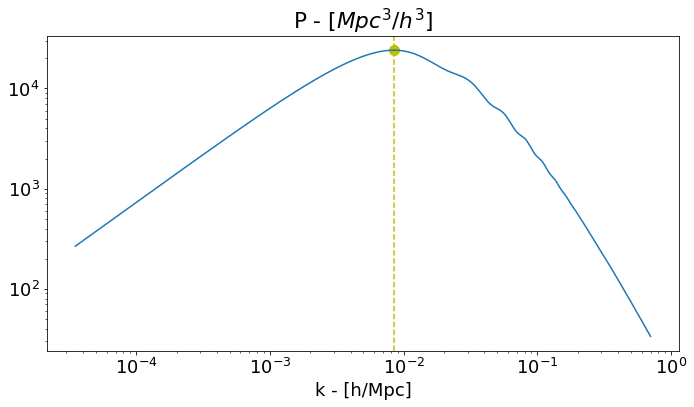
\includegraphics[scale=0.5]{../m4_figs/MatterPower.png}
    \caption{Matter power spectrum in $Mpc^3/h^3$. The "turnover point", corresponding to the peak of the spectrum, is marked at $k=\SI{0.012}{Mpc} = \SI{0.0084}{Mpc/h}$.}
    \label{fig:MatterPower}
\end{figure}



\subsection{Photon temperature power spectrum}
Figure \ref{fig:Cell} shown the temperature power spectrum, $C_\ell^{TT}$. 

\begin{figure}[h!]
    \centering
    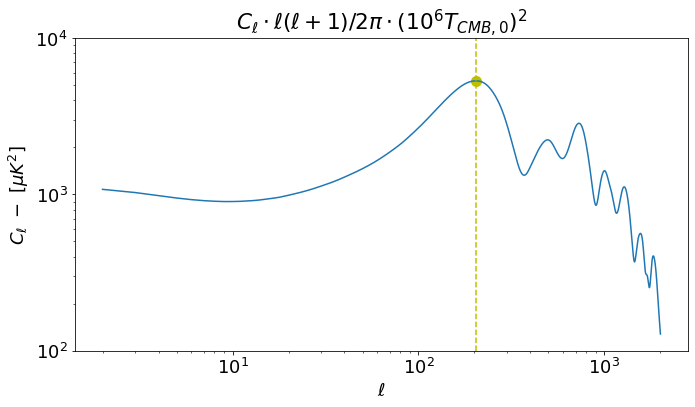
\includegraphics[scale=0.5]{../m4_figs/Cell.png}
    \caption{Photon temperature power spectrum, scaled by $\ell(\ell+1)/2\pi$, by convention, as function of $\ell$. The first maximum, at $\ell = 204$, is marked as a yellow point.}
    \label{fig:Cell}
\end{figure}

Figure \ref{fig:Cell_all} shows a decomposition of the temperature power spectrum into the four different contributing terms from the source function (equation \ref{eqn:source}). As we see, the Sachs-Wolfe term dominates at virtually all times, and decides all peaks and troughs in the power spectrum. The Doppler term also contributes a meaningful amount to the amplitude of the power spectrum, especially around $\ell=100$. We also see how the integrated Sachs-Wolfe effect contributes to the slight upwards slope towards very low $\ell$s. The quadrupole term is and should be completely negligible, but as far as I understand, the form of it is wrong. There is probably a bug somewhere in the calculation of the term.

\begin{figure}[h!]
    \centering
    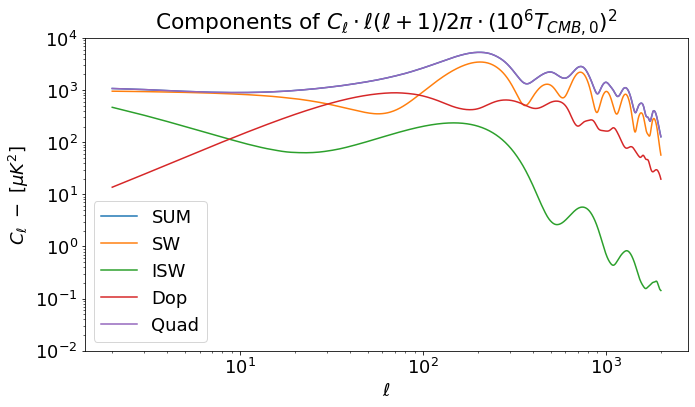
\includegraphics[scale=0.5]{../m4_figs/Cell_all.png}
    \caption{The same photon temperature power spectrum as in figure \ref{fig:Cell}, but separated into the four contributing terms from the source function.}
    \label{fig:Cell_all}
\end{figure}


\begin{figure}[h!]
    \centering
    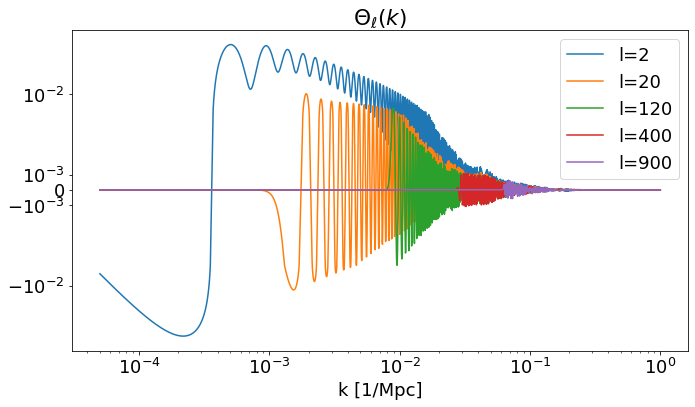
\includegraphics[scale=0.5]{../m4_figs/Theta.png}
    \caption{}
    \label{}
\end{figure}

\begin{figure}[h!]
    \centering
    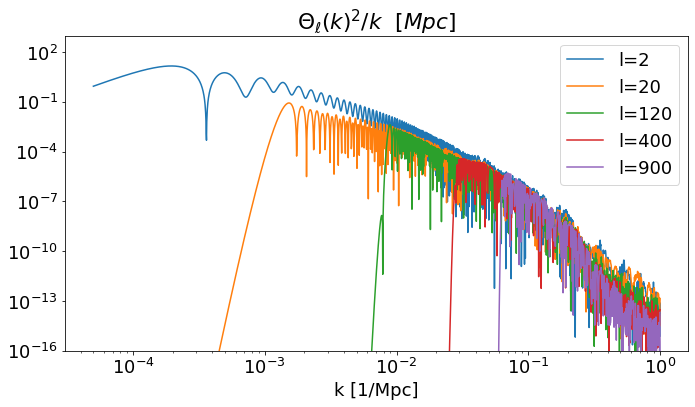
\includegraphics[scale=0.5]{../m4_figs/Theta2.png}
    \caption{}
    \label{}
\end{figure}



\newpage
\bibliography{ref}
\bibliographystyle{plain}



\end{document}